\titre{28}
\theme{trigo}
\auteur{Nathan Scheinmann}
\niveau{1M}
\source{sesamath-1M-trigo}
\type{serie}
\piments{2}
\pts{}
\annee{2425}

\contenu{
\tcblower 
On doit percer un tunner pour une nouvelle autoroute à travers une montagne de $3225~\text{m}$ de haut. À une distande de $2000~\text{m}$ de la base de la montagne l'angle d'élévation est de $36^\circ$. Sur l'autre face, l'angle d'élévation à une distance de $1500~\text{m}$ est de $60^\circ$. 
\begin{center}
	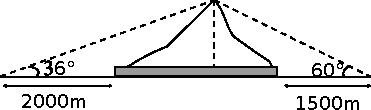
\includegraphics[scale=1]{../medias/1M/trigo/1M-exo-28}
\end{center}
Calculer la longueur du tunnel.

}
\correction{

}

